\documentclass{standalone}
\usepackage{tikz}
\usetikzlibrary{patterns}
\usetikzlibrary{positioning}
\usetikzlibrary{patterns, positioning}
\usetikzlibrary{shapes.misc}
\usepackage[outline]{contour}
\contourlength{1.5pt} 
\usetikzlibrary{calc}
        \usepackage{relsize}
        \tikzset{fontscale/.style = {font=\relsize{#1}}}

\begin{document}
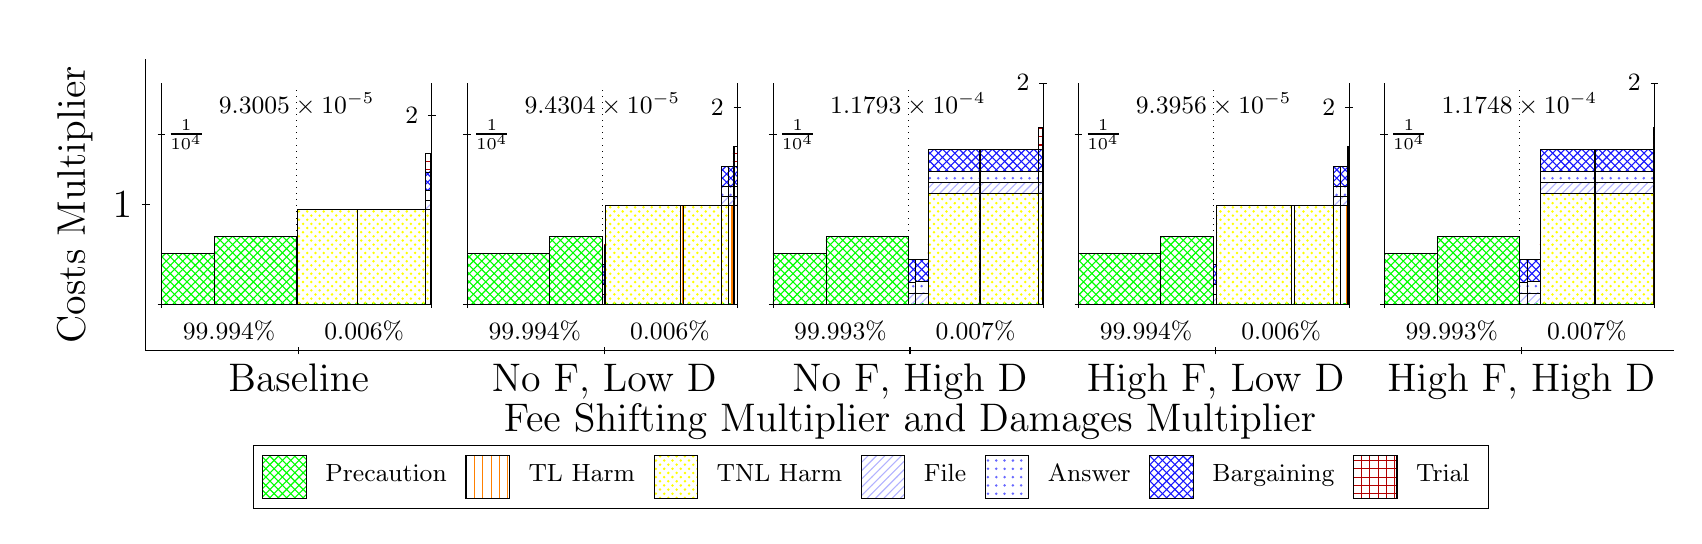
\begin{tikzpicture}
\clip(-0.5,-1.1) rectangle +(20.91,6.2);
\draw[black] (1,1) -- (1,4.7);
\node[rotate=90, fontscale=2, anchor=center] at (0.1, 2.85) {Costs Multiplier};
\draw[black] (0.95,2.85) -- (1.05,2.85);
\node[fontscale=2, anchor=east] at (0.95, 2.85) {1};

\draw[black] (1,1) -- (20.41,1);
\node[fontscale=2, anchor=center] at (10.705, 0.1) {Fee Shifting Multiplier and Damages Multiplier};
\draw[black] (2.941,0.95) -- (2.941,1.05);
\node[fontscale=2, anchor=north] at (2.941, 0.95) {Baseline};
\draw[black] (6.823,0.95) -- (6.823,1.05);
\node[fontscale=2, anchor=north] at (6.823, 0.95) {No F, Low D};
\draw[black] (10.705,0.95) -- (10.705,1.05);
\node[fontscale=2, anchor=north] at (10.705, 0.95) {No F, High D};
\draw[black] (14.587,0.95) -- (14.587,1.05);
\node[fontscale=2, anchor=north] at (14.587, 0.95) {High F, Low D};
\draw[black] (18.469,0.95) -- (18.469,1.05);
\node[fontscale=2, anchor=north] at (18.469, 0.95) {High F, High D};


\draw[pattern=crosshatch, pattern color=green,draw=black,very thin] (1.2,1.592) rectangle (1.8725,2.238);
\draw[pattern=crosshatch, pattern color=green,draw=black,very thin] (1.8725,1.592) rectangle (2.916,2.4534);
\draw[pattern=crosshatch, pattern color=green,draw=black,very thin] (2.916,1.592) rectangle (2.9287,1.592);
\draw[pattern=north east lines, pattern color=blue!30,draw=black,very thin] (2.916,1.592) rectangle (2.9287,1.7118);
\draw[pattern=dots,  pattern color=blue!60,draw=black,very thin] (2.916,1.7118) rectangle (2.9287,1.8315);
\draw[pattern=crosshatch,      pattern color=blue!90,draw=black,very thin] (2.916,1.8315) rectangle (2.9287,2.071);
\draw[pattern=grid,            pattern color=red!70!black,draw=black,very thin] (2.916,2.071) rectangle (2.9287,2.3105);
\draw[pattern=crosshatch, pattern color=green,draw=black,very thin] (2.9287,1.592) rectangle (3.6818,1.592);
\draw[pattern=crosshatch dots, pattern color=yellow,draw=black,very thin] (2.9287,1.592) rectangle (3.6818,2.7895);
\draw[pattern=crosshatch, pattern color=green,draw=black,very thin] (3.6818,1.592) rectangle (3.6897,1.592);
\draw[pattern=vertical lines, pattern color=orange,draw=black,very thin] (3.6818,1.592) rectangle (3.6897,2.7895);
\draw[pattern=crosshatch, pattern color=green,draw=black,very thin] (3.6897,1.592) rectangle (4.5556,1.592);
\draw[pattern=crosshatch dots, pattern color=yellow,draw=black,very thin] (3.6897,1.592) rectangle (4.5556,2.7895);
\draw[pattern=crosshatch, pattern color=green,draw=black,very thin] (4.5556,1.592) rectangle (4.6122,1.592);
\draw[pattern=crosshatch dots, pattern color=yellow,draw=black,very thin] (4.5556,1.592) rectangle (4.6122,2.7895);
\draw[pattern=north east lines, pattern color=blue!30,draw=black,very thin] (4.5556,2.7895) rectangle (4.6122,2.9093);
\draw[pattern=dots,  pattern color=blue!60,draw=black,very thin] (4.5556,2.9093) rectangle (4.6122,3.029);
\draw[pattern=crosshatch,      pattern color=blue!90,draw=black,very thin] (4.5556,3.029) rectangle (4.6122,3.2685);
\draw[pattern=grid,            pattern color=red!70!black,draw=black,very thin] (4.5556,3.2685) rectangle (4.6122,3.508);
\draw[pattern=crosshatch, pattern color=green,draw=black,very thin] (4.6122,1.592) rectangle (4.632,1.592);
\draw[pattern=vertical lines, pattern color=orange,draw=black,very thin] (4.6122,1.592) rectangle (4.632,2.7895);
\draw[pattern=north east lines, pattern color=blue!30,draw=black,very thin] (4.6122,2.7895) rectangle (4.632,2.9093);
\draw[pattern=dots,  pattern color=blue!60,draw=black,very thin] (4.6122,2.9093) rectangle (4.632,3.029);
\draw[pattern=crosshatch,      pattern color=blue!90,draw=black,very thin] (4.6122,3.029) rectangle (4.632,3.2685);
\draw[pattern=grid,            pattern color=red!70!black,draw=black,very thin] (4.6122,3.2685) rectangle (4.632,3.508);
\node[font=\small,text=black,anchor=north] at (2.916, 4.4) {$9.3005\times 10^{-5}$};
\draw[black,very thin] (1.2,1.592) -- (1.2,4.4);
\draw[black,very thin] (1.15,1.592) -- (1.25,1.592);
\node[font=\small,text=black, anchor=west] at (1.15, 1.592) {};
\draw[black,very thin] (1.15,3.7454) -- (1.25,3.7454);
\node[font=\small,text=black, anchor=west] at (1.15, 3.7454) {$\frac{1}{10^{4}}$};

\draw[black,dotted,very thin] (2.916,1.6762) -- (2.916,4.3158);
\draw[black,very thin] (4.632,1.592) -- (4.632,4.4);
\draw[black,very thin] (4.582,3.9869) -- (4.682,3.9869);
\node[font=\small,text=black, anchor=east] at (4.582, 3.9869) {\contour{white}{2}};

\draw[black,very thin] (1.2,1.592) -- (4.632,1.592);
\draw[black,very thin] (1.2,1.542) -- (1.2,1.642);
\node[font=\small,text=black, anchor=north] at (1.2, 1.542) {};
\draw[black,very thin] (4.632,1.542) -- (4.632,1.642);
\node[font=\small,text=black, anchor=north] at (4.632, 1.542) {};

\node[font=\small,text=black,anchor=south] at (2.058, 0.992) {99.994\%};
\node[font=\small,text=black,anchor=south] at (3.774, 0.992) {0.006\%};

\draw[pattern=crosshatch, pattern color=green,draw=black,very thin] (5.082,1.592) rectangle (6.1255,2.238);
\draw[pattern=crosshatch, pattern color=green,draw=black,very thin] (6.1255,1.592) rectangle (6.798,2.4534);
\draw[pattern=crosshatch, pattern color=green,draw=black,very thin] (6.798,1.592) rectangle (6.8222,1.592);
\draw[pattern=north east lines, pattern color=blue!30,draw=black,very thin] (6.798,1.592) rectangle (6.8222,1.7168);
\draw[pattern=dots,  pattern color=blue!60,draw=black,very thin] (6.798,1.7168) rectangle (6.8222,1.8416);
\draw[pattern=crosshatch,      pattern color=blue!90,draw=black,very thin] (6.798,1.8416) rectangle (6.8222,2.0911);
\draw[pattern=crosshatch, pattern color=green,draw=black,very thin] (6.8222,1.592) rectangle (6.8333,1.592);
\draw[pattern=north east lines, pattern color=blue!30,draw=black,very thin] (6.8222,1.592) rectangle (6.8333,1.7168);
\draw[pattern=dots,  pattern color=blue!60,draw=black,very thin] (6.8222,1.7168) rectangle (6.8333,1.8416);
\draw[pattern=crosshatch,      pattern color=blue!90,draw=black,very thin] (6.8222,1.8416) rectangle (6.8333,2.0911);
\draw[pattern=grid,            pattern color=red!70!black,draw=black,very thin] (6.8222,2.0911) rectangle (6.8333,2.3406);
\draw[pattern=crosshatch, pattern color=green,draw=black,very thin] (6.8333,1.592) rectangle (7.7841,1.592);
\draw[pattern=crosshatch dots, pattern color=yellow,draw=black,very thin] (6.8333,1.592) rectangle (7.7841,2.8396);
\draw[pattern=crosshatch, pattern color=green,draw=black,very thin] (7.7841,1.592) rectangle (7.8236,1.592);
\draw[pattern=vertical lines, pattern color=orange,draw=black,very thin] (7.7841,1.592) rectangle (7.8236,2.8396);
\draw[pattern=crosshatch, pattern color=green,draw=black,very thin] (7.8236,1.592) rectangle (8.3145,1.592);
\draw[pattern=crosshatch dots, pattern color=yellow,draw=black,very thin] (7.8236,1.592) rectangle (8.3145,2.8396);
\draw[pattern=crosshatch, pattern color=green,draw=black,very thin] (8.3145,1.592) rectangle (8.3974,1.592);
\draw[pattern=crosshatch dots, pattern color=yellow,draw=black,very thin] (8.3145,1.592) rectangle (8.3974,2.8396);
\draw[pattern=north east lines, pattern color=blue!30,draw=black,very thin] (8.3145,2.8396) rectangle (8.3974,2.9644);
\draw[pattern=dots,  pattern color=blue!60,draw=black,very thin] (8.3145,2.9644) rectangle (8.3974,3.0891);
\draw[pattern=crosshatch,      pattern color=blue!90,draw=black,very thin] (8.3145,3.0891) rectangle (8.3974,3.3387);
\draw[pattern=crosshatch, pattern color=green,draw=black,very thin] (8.3974,1.592) rectangle (8.4547,1.592);
\draw[pattern=vertical lines, pattern color=orange,draw=black,very thin] (8.3974,1.592) rectangle (8.4547,2.8396);
\draw[pattern=north east lines, pattern color=blue!30,draw=black,very thin] (8.3974,2.8396) rectangle (8.4547,2.9644);
\draw[pattern=dots,  pattern color=blue!60,draw=black,very thin] (8.3974,2.9644) rectangle (8.4547,3.0891);
\draw[pattern=crosshatch,      pattern color=blue!90,draw=black,very thin] (8.3974,3.0891) rectangle (8.4547,3.3387);
\draw[pattern=crosshatch, pattern color=green,draw=black,very thin] (8.4547,1.592) rectangle (8.4695,1.592);
\draw[pattern=crosshatch dots, pattern color=yellow,draw=black,very thin] (8.4547,1.592) rectangle (8.4695,2.8396);
\draw[pattern=north east lines, pattern color=blue!30,draw=black,very thin] (8.4547,2.8396) rectangle (8.4695,2.9644);
\draw[pattern=dots,  pattern color=blue!60,draw=black,very thin] (8.4547,2.9644) rectangle (8.4695,3.0891);
\draw[pattern=crosshatch,      pattern color=blue!90,draw=black,very thin] (8.4547,3.0891) rectangle (8.4695,3.3387);
\draw[pattern=grid,            pattern color=red!70!black,draw=black,very thin] (8.4547,3.3387) rectangle (8.4695,3.5882);
\draw[pattern=crosshatch, pattern color=green,draw=black,very thin] (8.4695,1.592) rectangle (8.514,1.592);
\draw[pattern=vertical lines, pattern color=orange,draw=black,very thin] (8.4695,1.592) rectangle (8.514,2.8396);
\draw[pattern=north east lines, pattern color=blue!30,draw=black,very thin] (8.4695,2.8396) rectangle (8.514,2.9644);
\draw[pattern=dots,  pattern color=blue!60,draw=black,very thin] (8.4695,2.9644) rectangle (8.514,3.0891);
\draw[pattern=crosshatch,      pattern color=blue!90,draw=black,very thin] (8.4695,3.0891) rectangle (8.514,3.3387);
\draw[pattern=grid,            pattern color=red!70!black,draw=black,very thin] (8.4695,3.3387) rectangle (8.514,3.5882);
\node[font=\small,text=black,anchor=north] at (6.798, 4.4) {$9.4304\times 10^{-5}$};
\draw[black,very thin] (5.082,1.592) -- (5.082,4.4);
\draw[black,very thin] (5.032,1.592) -- (5.132,1.592);
\node[font=\small,text=black, anchor=west] at (5.032, 1.592) {};
\draw[black,very thin] (5.032,3.7454) -- (5.132,3.7454);
\node[font=\small,text=black, anchor=west] at (5.032, 3.7454) {$\frac{1}{10^{4}}$};

\draw[black,dotted,very thin] (6.798,1.6762) -- (6.798,4.3158);
\draw[black,very thin] (8.514,1.592) -- (8.514,4.4);
\draw[black,very thin] (8.464,4.0872) -- (8.564,4.0872);
\node[font=\small,text=black, anchor=east] at (8.464, 4.0872) {\contour{white}{2}};

\draw[black,very thin] (5.082,1.592) -- (8.514,1.592);
\draw[black,very thin] (5.082,1.542) -- (5.082,1.642);
\node[font=\small,text=black, anchor=north] at (5.082, 1.542) {};
\draw[black,very thin] (8.514,1.542) -- (8.514,1.642);
\node[font=\small,text=black, anchor=north] at (8.514, 1.542) {};

\node[font=\small,text=black,anchor=south] at (5.94, 0.992) {99.994\%};
\node[font=\small,text=black,anchor=south] at (7.656, 0.992) {0.006\%};

\draw[pattern=crosshatch, pattern color=green,draw=black,very thin] (8.964,1.592) rectangle (9.6365,2.238);
\draw[pattern=crosshatch, pattern color=green,draw=black,very thin] (9.6365,1.592) rectangle (10.68,2.4534);
\draw[pattern=crosshatch, pattern color=green,draw=black,very thin] (10.68,1.592) rectangle (10.772,1.592);
\draw[pattern=north east lines, pattern color=blue!30,draw=black,very thin] (10.68,1.592) rectangle (10.772,1.7324);
\draw[pattern=dots,  pattern color=blue!60,draw=black,very thin] (10.68,1.7324) rectangle (10.772,1.8728);
\draw[pattern=crosshatch,      pattern color=blue!90,draw=black,very thin] (10.68,1.8728) rectangle (10.772,2.1536);
\draw[pattern=crosshatch, pattern color=green,draw=black,very thin] (10.772,1.592) rectangle (10.932,1.5921);
\draw[pattern=north east lines, pattern color=blue!30,draw=black,very thin] (10.772,1.5921) rectangle (10.932,1.7325);
\draw[pattern=dots,  pattern color=blue!60,draw=black,very thin] (10.772,1.7325) rectangle (10.932,1.8729);
\draw[pattern=crosshatch,      pattern color=blue!90,draw=black,very thin] (10.772,1.8729) rectangle (10.932,2.1536);
\draw[pattern=crosshatch, pattern color=green,draw=black,very thin] (10.932,1.592) rectangle (10.943,1.592);
\draw[pattern=north east lines, pattern color=blue!30,draw=black,very thin] (10.932,1.592) rectangle (10.943,1.7324);
\draw[pattern=dots,  pattern color=blue!60,draw=black,very thin] (10.932,1.7324) rectangle (10.943,1.8728);
\draw[pattern=crosshatch,      pattern color=blue!90,draw=black,very thin] (10.932,1.8728) rectangle (10.943,2.1536);
\draw[pattern=grid,            pattern color=red!70!black,draw=black,very thin] (10.932,2.1536) rectangle (10.943,2.4344);
\draw[pattern=crosshatch, pattern color=green,draw=black,very thin] (10.943,1.592) rectangle (11.586,1.592);
\draw[pattern=crosshatch dots, pattern color=yellow,draw=black,very thin] (10.943,1.592) rectangle (11.586,2.996);
\draw[pattern=north east lines, pattern color=blue!30,draw=black,very thin] (10.943,2.996) rectangle (11.586,3.1364);
\draw[pattern=dots,  pattern color=blue!60,draw=black,very thin] (10.943,3.1364) rectangle (11.586,3.2768);
\draw[pattern=crosshatch,      pattern color=blue!90,draw=black,very thin] (10.943,3.2768) rectangle (11.586,3.5576);
\draw[pattern=crosshatch, pattern color=green,draw=black,very thin] (11.586,1.592) rectangle (11.592,1.592);
\draw[pattern=vertical lines, pattern color=orange,draw=black,very thin] (11.586,1.592) rectangle (11.592,2.996);
\draw[pattern=north east lines, pattern color=blue!30,draw=black,very thin] (11.586,2.996) rectangle (11.592,3.1364);
\draw[pattern=dots,  pattern color=blue!60,draw=black,very thin] (11.586,3.1364) rectangle (11.592,3.2768);
\draw[pattern=crosshatch,      pattern color=blue!90,draw=black,very thin] (11.586,3.2768) rectangle (11.592,3.5576);
\draw[pattern=crosshatch, pattern color=green,draw=black,very thin] (11.592,1.592) rectangle (12.331,1.5921);
\draw[pattern=crosshatch dots, pattern color=yellow,draw=black,very thin] (11.592,1.5921) rectangle (12.331,2.996);
\draw[pattern=north east lines, pattern color=blue!30,draw=black,very thin] (11.592,2.996) rectangle (12.331,3.1364);
\draw[pattern=dots,  pattern color=blue!60,draw=black,very thin] (11.592,3.1364) rectangle (12.331,3.2768);
\draw[pattern=crosshatch,      pattern color=blue!90,draw=black,very thin] (11.592,3.2768) rectangle (12.331,3.5576);
\draw[pattern=crosshatch, pattern color=green,draw=black,very thin] (12.331,1.592) rectangle (12.379,1.592);
\draw[pattern=crosshatch dots, pattern color=yellow,draw=black,very thin] (12.331,1.592) rectangle (12.379,2.996);
\draw[pattern=north east lines, pattern color=blue!30,draw=black,very thin] (12.331,2.996) rectangle (12.379,3.1364);
\draw[pattern=dots,  pattern color=blue!60,draw=black,very thin] (12.331,3.1364) rectangle (12.379,3.2768);
\draw[pattern=crosshatch,      pattern color=blue!90,draw=black,very thin] (12.331,3.2768) rectangle (12.379,3.5576);
\draw[pattern=grid,            pattern color=red!70!black,draw=black,very thin] (12.331,3.5576) rectangle (12.379,3.8384);
\draw[pattern=crosshatch, pattern color=green,draw=black,very thin] (12.379,1.592) rectangle (12.396,1.592);
\draw[pattern=vertical lines, pattern color=orange,draw=black,very thin] (12.379,1.592) rectangle (12.396,2.996);
\draw[pattern=north east lines, pattern color=blue!30,draw=black,very thin] (12.379,2.996) rectangle (12.396,3.1364);
\draw[pattern=dots,  pattern color=blue!60,draw=black,very thin] (12.379,3.1364) rectangle (12.396,3.2768);
\draw[pattern=crosshatch,      pattern color=blue!90,draw=black,very thin] (12.379,3.2768) rectangle (12.396,3.5576);
\draw[pattern=grid,            pattern color=red!70!black,draw=black,very thin] (12.379,3.5576) rectangle (12.396,3.8384);
\node[font=\small,text=black,anchor=north] at (10.68, 4.4) {$1.1793\times 10^{-4}$};
\draw[black,very thin] (8.964,1.592) -- (8.964,4.4);
\draw[black,very thin] (8.914,1.592) -- (9.014,1.592);
\node[font=\small,text=black, anchor=west] at (8.914, 1.592) {};
\draw[black,very thin] (8.914,3.7454) -- (9.014,3.7454);
\node[font=\small,text=black, anchor=west] at (8.914, 3.7454) {$\frac{1}{10^{4}}$};

\draw[black,dotted,very thin] (10.68,1.6762) -- (10.68,4.3158);
\draw[black,very thin] (12.396,1.592) -- (12.396,4.4);
\draw[black,very thin] (12.346,4.3999) -- (12.446,4.3999);
\node[font=\small,text=black, anchor=east] at (12.346, 4.3999) {\contour{white}{2}};

\draw[black,very thin] (8.964,1.592) -- (12.396,1.592);
\draw[black,very thin] (8.964,1.542) -- (8.964,1.642);
\node[font=\small,text=black, anchor=north] at (8.964, 1.542) {};
\draw[black,very thin] (12.396,1.542) -- (12.396,1.642);
\node[font=\small,text=black, anchor=north] at (12.396, 1.542) {};

\node[font=\small,text=black,anchor=south] at (9.822, 0.992) {99.993\%};
\node[font=\small,text=black,anchor=south] at (11.538, 0.992) {0.007\%};

\draw[pattern=crosshatch, pattern color=green,draw=black,very thin] (12.846,1.592) rectangle (13.89,2.238);
\draw[pattern=crosshatch, pattern color=green,draw=black,very thin] (13.89,1.592) rectangle (14.562,2.4534);
\draw[pattern=crosshatch, pattern color=green,draw=black,very thin] (14.562,1.592) rectangle (14.595,1.592);
\draw[pattern=north east lines, pattern color=blue!30,draw=black,very thin] (14.562,1.592) rectangle (14.595,1.7168);
\draw[pattern=dots,  pattern color=blue!60,draw=black,very thin] (14.562,1.7168) rectangle (14.595,1.8416);
\draw[pattern=crosshatch,      pattern color=blue!90,draw=black,very thin] (14.562,1.8416) rectangle (14.595,2.0911);
\draw[pattern=crosshatch, pattern color=green,draw=black,very thin] (14.595,1.592) rectangle (14.597,1.592);
\draw[pattern=north east lines, pattern color=blue!30,draw=black,very thin] (14.595,1.592) rectangle (14.597,1.7168);
\draw[pattern=dots,  pattern color=blue!60,draw=black,very thin] (14.595,1.7168) rectangle (14.597,1.8416);
\draw[pattern=crosshatch,      pattern color=blue!90,draw=black,very thin] (14.595,1.8416) rectangle (14.597,2.0911);
\draw[pattern=grid,            pattern color=red!70!black,draw=black,very thin] (14.595,2.0911) rectangle (14.597,2.3406);
\draw[pattern=crosshatch, pattern color=green,draw=black,very thin] (14.597,1.592) rectangle (15.548,1.592);
\draw[pattern=crosshatch dots, pattern color=yellow,draw=black,very thin] (14.597,1.592) rectangle (15.548,2.8397);
\draw[pattern=crosshatch, pattern color=green,draw=black,very thin] (15.548,1.592) rectangle (15.588,1.592);
\draw[pattern=vertical lines, pattern color=orange,draw=black,very thin] (15.548,1.592) rectangle (15.588,2.8397);
\draw[pattern=crosshatch, pattern color=green,draw=black,very thin] (15.588,1.592) rectangle (16.078,1.592);
\draw[pattern=crosshatch dots, pattern color=yellow,draw=black,very thin] (15.588,1.592) rectangle (16.078,2.8397);
\draw[pattern=crosshatch, pattern color=green,draw=black,very thin] (16.078,1.592) rectangle (16.168,1.592);
\draw[pattern=crosshatch dots, pattern color=yellow,draw=black,very thin] (16.078,1.592) rectangle (16.168,2.8397);
\draw[pattern=north east lines, pattern color=blue!30,draw=black,very thin] (16.078,2.8397) rectangle (16.168,2.9644);
\draw[pattern=dots,  pattern color=blue!60,draw=black,very thin] (16.078,2.9644) rectangle (16.168,3.0892);
\draw[pattern=crosshatch,      pattern color=blue!90,draw=black,very thin] (16.078,3.0892) rectangle (16.168,3.3387);
\draw[pattern=crosshatch, pattern color=green,draw=black,very thin] (16.168,1.592) rectangle (16.262,1.592);
\draw[pattern=vertical lines, pattern color=orange,draw=black,very thin] (16.168,1.592) rectangle (16.262,2.8397);
\draw[pattern=north east lines, pattern color=blue!30,draw=black,very thin] (16.168,2.8397) rectangle (16.262,2.9644);
\draw[pattern=dots,  pattern color=blue!60,draw=black,very thin] (16.168,2.9644) rectangle (16.262,3.0892);
\draw[pattern=crosshatch,      pattern color=blue!90,draw=black,very thin] (16.168,3.0892) rectangle (16.262,3.3387);
\draw[pattern=crosshatch, pattern color=green,draw=black,very thin] (16.262,1.592) rectangle (16.27,1.592);
\draw[pattern=crosshatch dots, pattern color=yellow,draw=black,very thin] (16.262,1.592) rectangle (16.27,2.8397);
\draw[pattern=north east lines, pattern color=blue!30,draw=black,very thin] (16.262,2.8397) rectangle (16.27,2.9644);
\draw[pattern=dots,  pattern color=blue!60,draw=black,very thin] (16.262,2.9644) rectangle (16.27,3.0892);
\draw[pattern=crosshatch,      pattern color=blue!90,draw=black,very thin] (16.262,3.0892) rectangle (16.27,3.3387);
\draw[pattern=grid,            pattern color=red!70!black,draw=black,very thin] (16.262,3.3387) rectangle (16.27,3.5882);
\draw[pattern=crosshatch, pattern color=green,draw=black,very thin] (16.27,1.592) rectangle (16.278,1.592);
\draw[pattern=vertical lines, pattern color=orange,draw=black,very thin] (16.27,1.592) rectangle (16.278,2.8397);
\draw[pattern=north east lines, pattern color=blue!30,draw=black,very thin] (16.27,2.8397) rectangle (16.278,2.9644);
\draw[pattern=dots,  pattern color=blue!60,draw=black,very thin] (16.27,2.9644) rectangle (16.278,3.0892);
\draw[pattern=crosshatch,      pattern color=blue!90,draw=black,very thin] (16.27,3.0892) rectangle (16.278,3.3387);
\draw[pattern=grid,            pattern color=red!70!black,draw=black,very thin] (16.27,3.3387) rectangle (16.278,3.5882);
\node[font=\small,text=black,anchor=north] at (14.562, 4.4) {$9.3956\times 10^{-5}$};
\draw[black,very thin] (12.846,1.592) -- (12.846,4.4);
\draw[black,very thin] (12.796,1.592) -- (12.896,1.592);
\node[font=\small,text=black, anchor=west] at (12.796, 1.592) {};
\draw[black,very thin] (12.796,3.7454) -- (12.896,3.7454);
\node[font=\small,text=black, anchor=west] at (12.796, 3.7454) {$\frac{1}{10^{4}}$};

\draw[black,dotted,very thin] (14.562,1.6762) -- (14.562,4.3158);
\draw[black,very thin] (16.278,1.592) -- (16.278,4.4);
\draw[black,very thin] (16.228,4.0872) -- (16.328,4.0872);
\node[font=\small,text=black, anchor=east] at (16.228, 4.0872) {\contour{white}{2}};

\draw[black,very thin] (12.846,1.592) -- (16.278,1.592);
\draw[black,very thin] (12.846,1.542) -- (12.846,1.642);
\node[font=\small,text=black, anchor=north] at (12.846, 1.542) {};
\draw[black,very thin] (16.278,1.542) -- (16.278,1.642);
\node[font=\small,text=black, anchor=north] at (16.278, 1.542) {};

\node[font=\small,text=black,anchor=south] at (13.704, 0.992) {99.994\%};
\node[font=\small,text=black,anchor=south] at (15.42, 0.992) {0.006\%};

\draw[pattern=crosshatch, pattern color=green,draw=black,very thin] (16.728,1.592) rectangle (17.4,2.238);
\draw[pattern=crosshatch, pattern color=green,draw=black,very thin] (17.4,1.592) rectangle (18.444,2.4534);
\draw[pattern=crosshatch, pattern color=green,draw=black,very thin] (18.444,1.592) rectangle (18.545,1.592);
\draw[pattern=north east lines, pattern color=blue!30,draw=black,very thin] (18.444,1.592) rectangle (18.545,1.7324);
\draw[pattern=dots,  pattern color=blue!60,draw=black,very thin] (18.444,1.7324) rectangle (18.545,1.8728);
\draw[pattern=crosshatch,      pattern color=blue!90,draw=black,very thin] (18.444,1.8728) rectangle (18.545,2.1536);
\draw[pattern=crosshatch, pattern color=green,draw=black,very thin] (18.545,1.592) rectangle (18.705,1.5921);
\draw[pattern=north east lines, pattern color=blue!30,draw=black,very thin] (18.545,1.5921) rectangle (18.705,1.7325);
\draw[pattern=dots,  pattern color=blue!60,draw=black,very thin] (18.545,1.7325) rectangle (18.705,1.8729);
\draw[pattern=crosshatch,      pattern color=blue!90,draw=black,very thin] (18.545,1.8729) rectangle (18.705,2.1536);
\draw[pattern=crosshatch, pattern color=green,draw=black,very thin] (18.705,1.592) rectangle (18.707,1.592);
\draw[pattern=north east lines, pattern color=blue!30,draw=black,very thin] (18.705,1.592) rectangle (18.707,1.7324);
\draw[pattern=dots,  pattern color=blue!60,draw=black,very thin] (18.705,1.7324) rectangle (18.707,1.8728);
\draw[pattern=crosshatch,      pattern color=blue!90,draw=black,very thin] (18.705,1.8728) rectangle (18.707,2.1536);
\draw[pattern=grid,            pattern color=red!70!black,draw=black,very thin] (18.705,2.1536) rectangle (18.707,2.4344);
\draw[pattern=crosshatch, pattern color=green,draw=black,very thin] (18.707,1.592) rectangle (19.391,1.592);
\draw[pattern=crosshatch dots, pattern color=yellow,draw=black,very thin] (18.707,1.592) rectangle (19.391,2.996);
\draw[pattern=north east lines, pattern color=blue!30,draw=black,very thin] (18.707,2.996) rectangle (19.391,3.1364);
\draw[pattern=dots,  pattern color=blue!60,draw=black,very thin] (18.707,3.1364) rectangle (19.391,3.2768);
\draw[pattern=crosshatch,      pattern color=blue!90,draw=black,very thin] (18.707,3.2768) rectangle (19.391,3.5576);
\draw[pattern=crosshatch, pattern color=green,draw=black,very thin] (19.391,1.592) rectangle (19.407,1.592);
\draw[pattern=vertical lines, pattern color=orange,draw=black,very thin] (19.391,1.592) rectangle (19.407,2.996);
\draw[pattern=north east lines, pattern color=blue!30,draw=black,very thin] (19.391,2.996) rectangle (19.407,3.1364);
\draw[pattern=dots,  pattern color=blue!60,draw=black,very thin] (19.391,3.1364) rectangle (19.407,3.2768);
\draw[pattern=crosshatch,      pattern color=blue!90,draw=black,very thin] (19.391,3.2768) rectangle (19.407,3.5576);
\draw[pattern=crosshatch, pattern color=green,draw=black,very thin] (19.407,1.592) rectangle (20.146,1.5921);
\draw[pattern=crosshatch dots, pattern color=yellow,draw=black,very thin] (19.407,1.5921) rectangle (20.146,2.996);
\draw[pattern=north east lines, pattern color=blue!30,draw=black,very thin] (19.407,2.996) rectangle (20.146,3.1364);
\draw[pattern=dots,  pattern color=blue!60,draw=black,very thin] (19.407,3.1364) rectangle (20.146,3.2768);
\draw[pattern=crosshatch,      pattern color=blue!90,draw=black,very thin] (19.407,3.2768) rectangle (20.146,3.5576);
\draw[pattern=crosshatch, pattern color=green,draw=black,very thin] (20.146,1.592) rectangle (20.153,1.592);
\draw[pattern=crosshatch dots, pattern color=yellow,draw=black,very thin] (20.146,1.592) rectangle (20.153,2.996);
\draw[pattern=north east lines, pattern color=blue!30,draw=black,very thin] (20.146,2.996) rectangle (20.153,3.1364);
\draw[pattern=dots,  pattern color=blue!60,draw=black,very thin] (20.146,3.1364) rectangle (20.153,3.2768);
\draw[pattern=crosshatch,      pattern color=blue!90,draw=black,very thin] (20.146,3.2768) rectangle (20.153,3.5576);
\draw[pattern=grid,            pattern color=red!70!black,draw=black,very thin] (20.146,3.5576) rectangle (20.153,3.8384);
\draw[pattern=crosshatch, pattern color=green,draw=black,very thin] (20.153,1.592) rectangle (20.16,1.592);
\draw[pattern=vertical lines, pattern color=orange,draw=black,very thin] (20.153,1.592) rectangle (20.16,2.996);
\draw[pattern=north east lines, pattern color=blue!30,draw=black,very thin] (20.153,2.996) rectangle (20.16,3.1364);
\draw[pattern=dots,  pattern color=blue!60,draw=black,very thin] (20.153,3.1364) rectangle (20.16,3.2768);
\draw[pattern=crosshatch,      pattern color=blue!90,draw=black,very thin] (20.153,3.2768) rectangle (20.16,3.5576);
\draw[pattern=grid,            pattern color=red!70!black,draw=black,very thin] (20.153,3.5576) rectangle (20.16,3.8384);
\node[font=\small,text=black,anchor=north] at (18.444, 4.4) {$1.1748\times 10^{-4}$};
\draw[black,very thin] (16.728,1.592) -- (16.728,4.4);
\draw[black,very thin] (16.678,1.592) -- (16.778,1.592);
\node[font=\small,text=black, anchor=west] at (16.678, 1.592) {};
\draw[black,very thin] (16.678,3.7454) -- (16.778,3.7454);
\node[font=\small,text=black, anchor=west] at (16.678, 3.7454) {$\frac{1}{10^{4}}$};

\draw[black,dotted,very thin] (18.444,1.6762) -- (18.444,4.3158);
\draw[black,very thin] (20.16,1.592) -- (20.16,4.4);
\draw[black,very thin] (20.11,4.3999) -- (20.21,4.3999);
\node[font=\small,text=black, anchor=east] at (20.11, 4.3999) {\contour{white}{2}};

\draw[black,very thin] (16.728,1.592) -- (20.16,1.592);
\draw[black,very thin] (16.728,1.542) -- (16.728,1.642);
\node[font=\small,text=black, anchor=north] at (16.728, 1.542) {};
\draw[black,very thin] (20.16,1.542) -- (20.16,1.642);
\node[font=\small,text=black, anchor=north] at (20.16, 1.542) {};

\node[font=\small,text=black,anchor=south] at (17.586, 0.992) {99.993\%};
\node[font=\small,text=black,anchor=south] at (19.302, 0.992) {0.007\%};

\coordinate (LegendAnchor) at (10.205000000000002,0);
\begin{scope}[align=center]
\matrix[scale=0.6,draw=black,below=0.2cm of LegendAnchor,nodes={draw},column sep=0.12cm]{
\node[rectangle,draw,minimum width=0.55cm,minimum height=0.55cm,pattern=crosshatch, pattern color=green]{}; &
        \node[draw=none,font=\small]{Precaution}; &
\node[rectangle,draw,minimum width=0.55cm,minimum height=0.55cm,pattern=vertical lines, pattern color=orange]{}; &
        \node[draw=none,font=\small]{TL Harm}; &
\node[rectangle,draw,minimum width=0.55cm,minimum height=0.55cm,pattern=crosshatch dots, pattern color=yellow]{}; &
        \node[draw=none,font=\small]{TNL Harm}; &
\node[rectangle,draw,minimum width=0.55cm,minimum height=0.55cm,pattern=north east lines, pattern color=blue!30]{}; &
        \node[draw=none,font=\small]{File}; &
\node[rectangle,draw,minimum width=0.55cm,minimum height=0.55cm,pattern=dots, pattern color=blue!60]{}; &
        \node[draw=none,font=\small]{Answer}; &
\node[rectangle,draw,minimum width=0.55cm,minimum height=0.55cm,pattern=crosshatch, pattern color=blue!90]{}; &
        \node[draw=none,font=\small]{Bargaining}; &
\node[rectangle,draw,minimum width=0.55cm,minimum height=0.55cm,pattern=grid, pattern color=red!70!black]{}; &
        \node[draw=none,font=\small]{Trial}; \\
};\end{scope}

\end{tikzpicture}
\end{document}